\documentclass{beamer}
\usetheme{Madrid}
\usecolortheme{default}

% Keep the original footer template
\setbeamertemplate{footline}{
  \leavevmode%
  \hbox{%
  \begin{beamercolorbox}[wd=.1\paperwidth,ht=2.25ex,dp=1ex,center]{date in head/foot}%
    
\includegraphics[height=2ex]{ua_logo.png}
  \end{beamercolorbox}%
  \begin{beamercolorbox}[wd=.8\paperwidth,ht=2.25ex,dp=1ex,center]{title in head/foot}%
    \usebeamerfont{title in head/foot}\insertshorttitle
  \end{beamercolorbox}%
  \begin{beamercolorbox}[wd=.1\paperwidth,ht=2.25ex,dp=1ex,right]{date in head/foot}%
    \usebeamerfont{date in head/foot}\insertframenumber{}/\inserttotalframenumber\hspace*{2ex}
  \end{beamercolorbox}}%
  \vskip0pt%
}

\title{Sign Language Recognition Using Neural Networks}
\subtitle{A Two-Layer Implementation for Static Gesture Recognition}
\author{Oleksandr Solovei}
\institute{Universidade de Aveiro}
\date{\today}

\begin{document}

\begin{frame}
    \titlepage
\end{frame}

\begin{frame}{Overview}
    \tableofcontents
\end{frame}

\section{Introduction}

\begin{frame}{Problem Statement \& Motivation}
    \begin{itemize}
        \item \textbf{Goal:} Develop an accessible sign language recognition system
        \item \textbf{Approach:} Two-layer neural network for static gesture classification
        \item \textbf{Dataset:} Sign Language MNIST
        \begin{itemize}
            \item 27,455 training images
            \item 7,172 test images
            \item 24 ASL letters (excluding J, Z which require motion)
        \end{itemize}
        \item \textbf{Impact:} Enhanced communication tools for deaf community
    \end{itemize}
\end{frame}

\section{Data Analysis}

\begin{frame}{Dataset Characteristics}
    \centering
    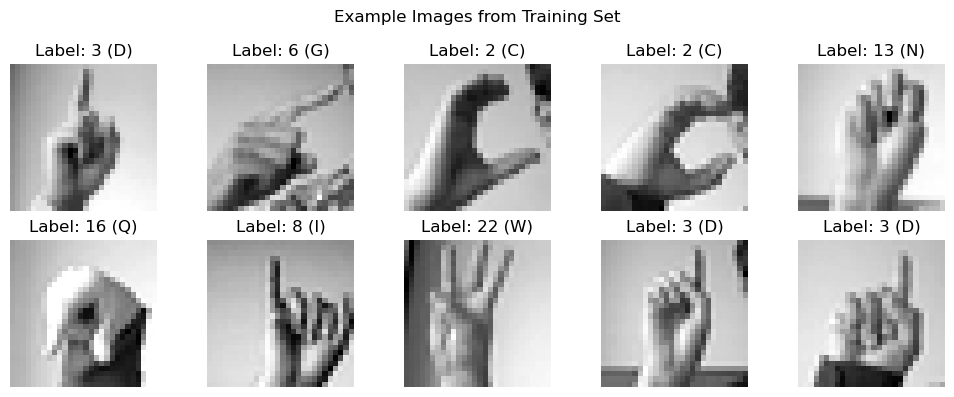
\includegraphics[width=0.8\textwidth]{dataset_sample.png}
    \begin{itemize}
        \begin{itemize}
            \item 28×28 grayscale images (784 features)
            \item Centered hand gestures
            \item Varying lighting conditions
        \end{itemize}
    \end{itemize}
\end{frame}

\begin{frame}{Dataset Distribution}
\centering
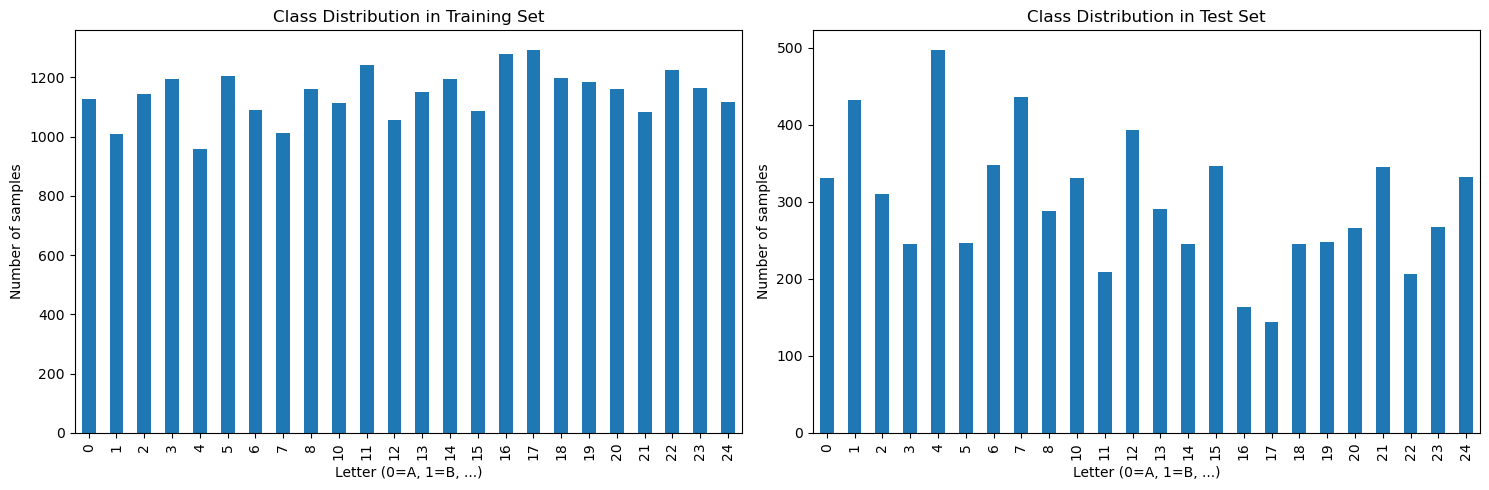
\includegraphics[width=0.8\textwidth]{dataset_distribution.png}
\begin{itemize}
    \item  \begin{center} Imbalanced classes (144-498 samples per class) \end{center}
    \item  \begin{center} Most frequent: Letter E (498 samples)
    \end{center}
    \item  \begin{center} Least frequent: Letter Q (144 samples)
    \end{center}
\end{itemize}
\end{frame}

\begin{frame}{Dataset Examples}
\centering
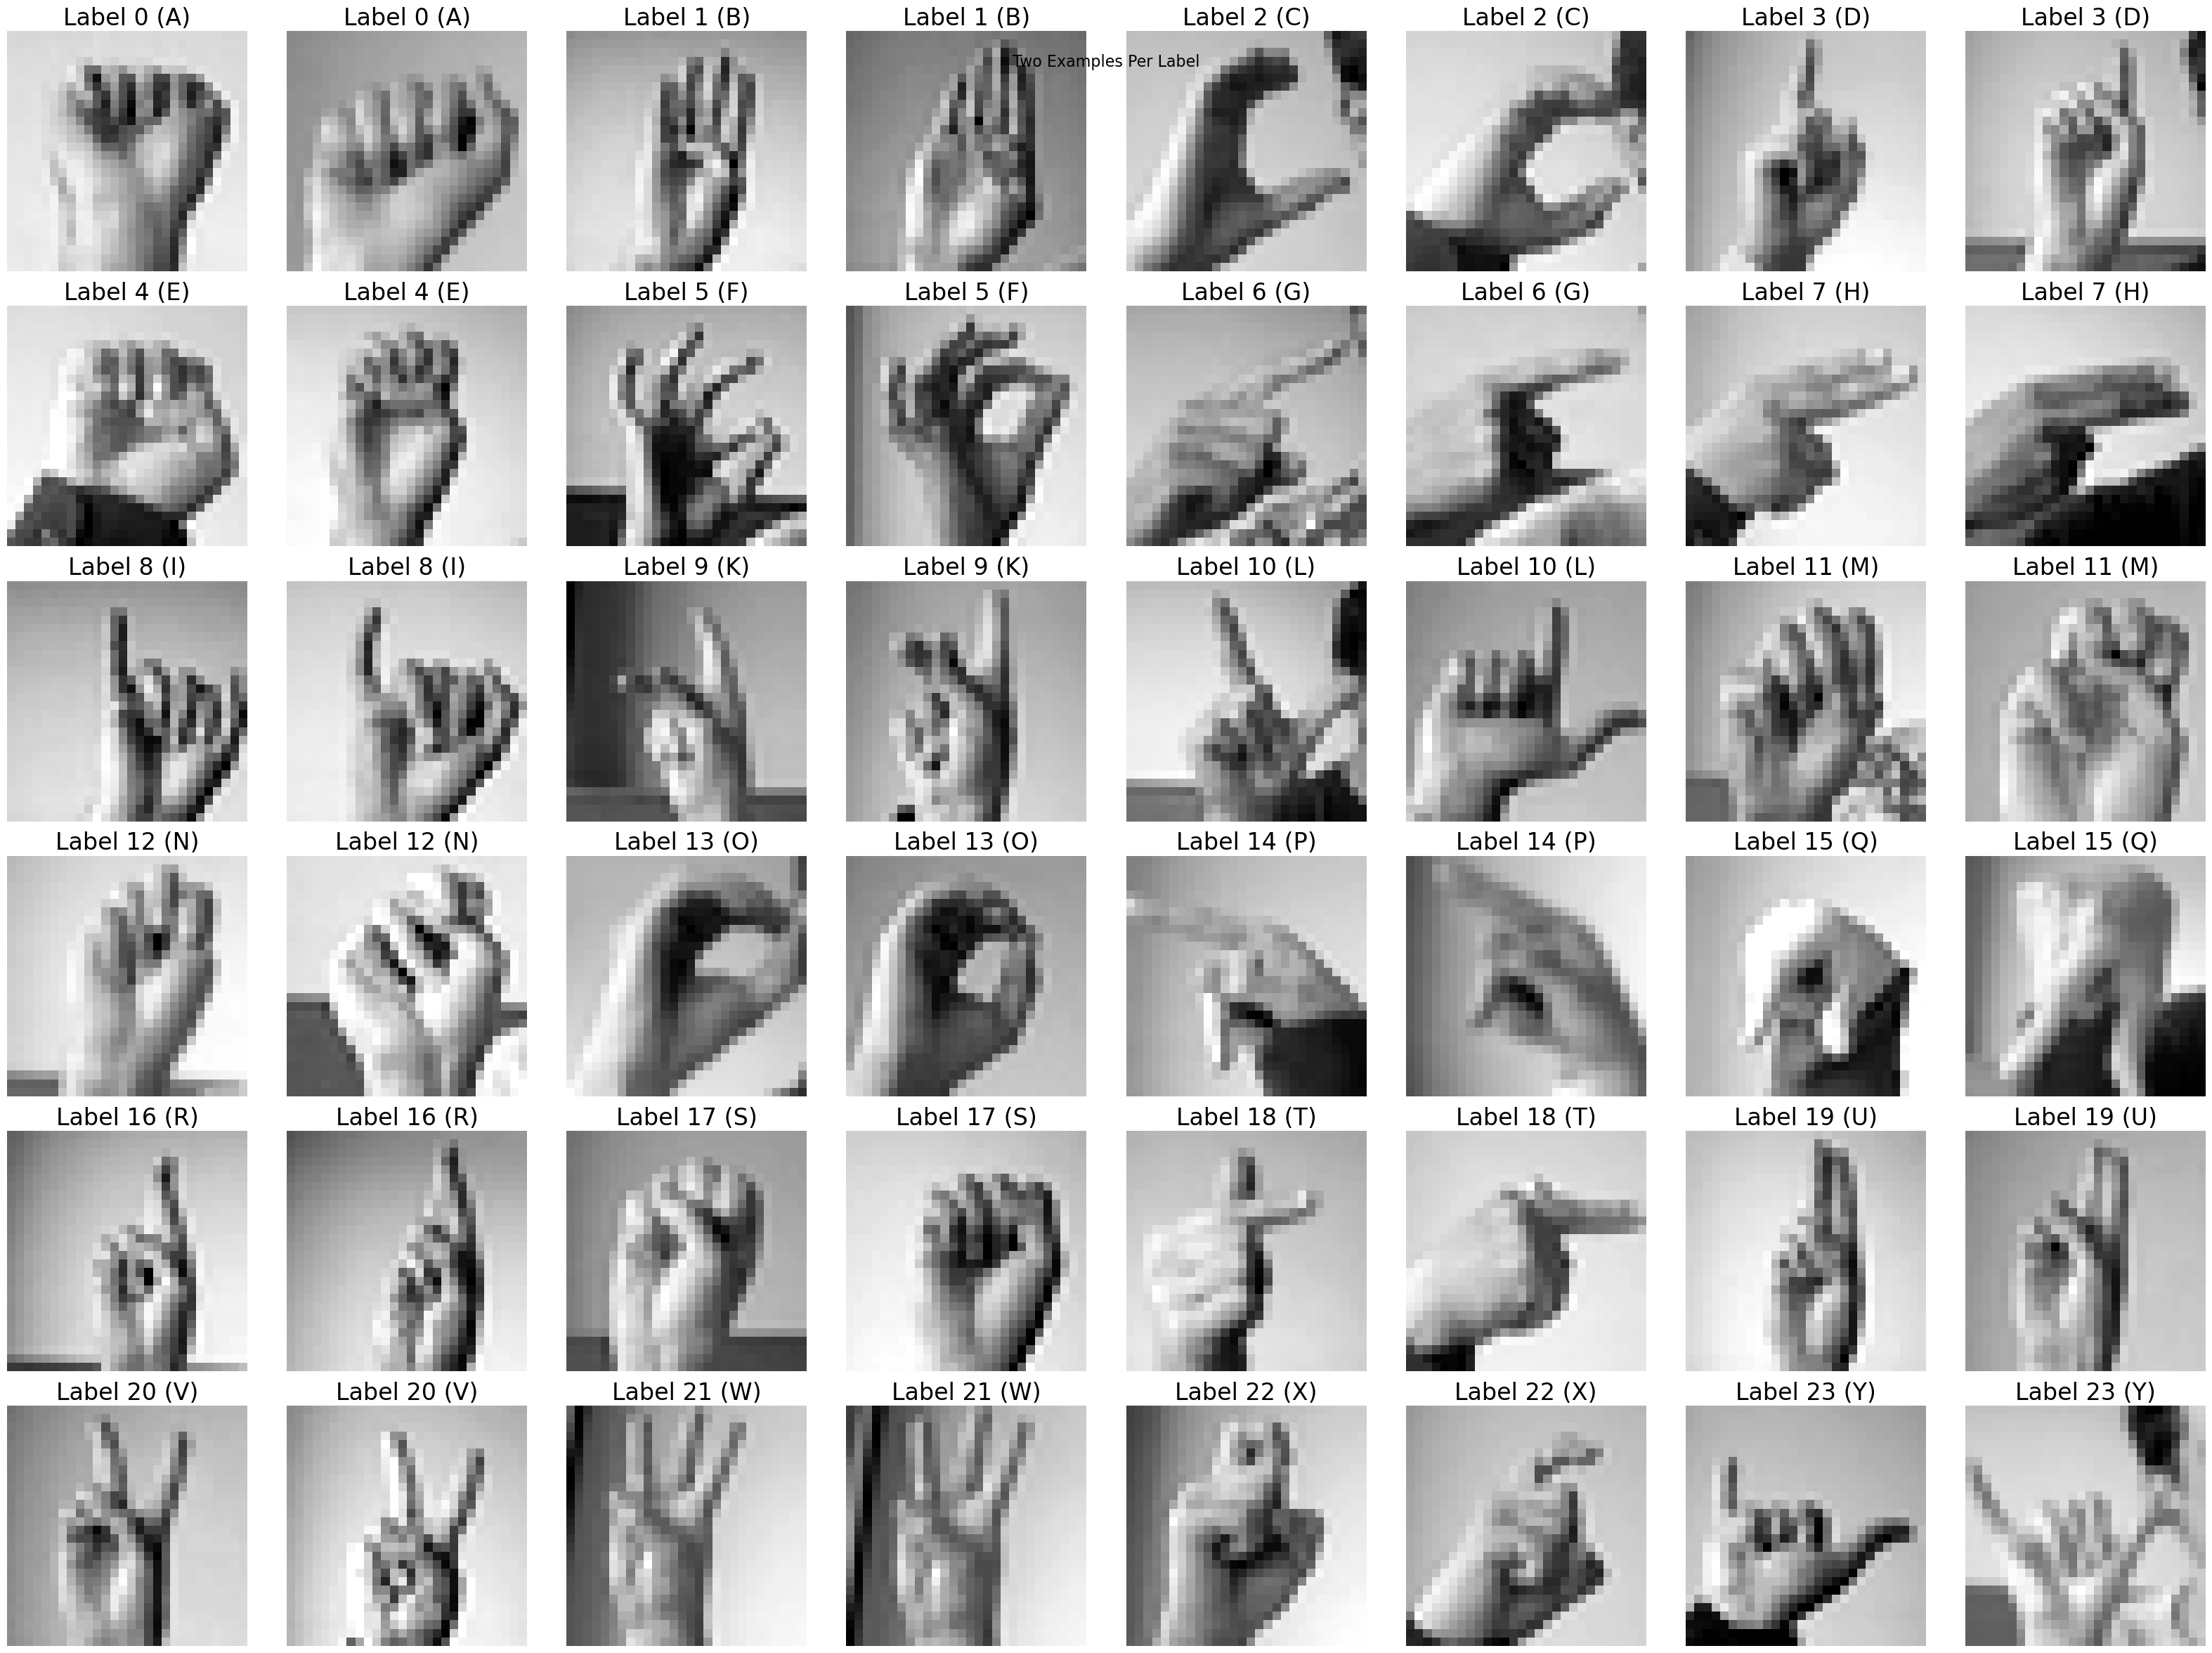
\includegraphics[width=0.8\textwidth]{dataset_items.png}
\end{frame}

\begin{frame}{Preprocessing Pipeline}
    \begin{itemize}
        \item \textbf{Data Normalization}
        \begin{itemize}
            \item Pixel scaling: $X_{normalized} = \frac{X}{255}$
            \item Range: [0, 1]
        \end{itemize}
        \item \textbf{Label Processing}
        \begin{itemize}
            \item One-hot encoding (24 classes)
            \item Label adjustment for J, Z gaps
        \end{itemize}
        \item \textbf{Data Splitting}
        \begin{itemize}
            \item Training Set: 27,455 samples
            \item Testing Set: 7,172 samples
        \end{itemize}
    \end{itemize}
\end{frame}

\section{Neural Network Architecture}

\begin{frame}{Model Architecture}
    \begin{itemize}
        \item \textbf{Network Structure}
        \begin{itemize}
            \item Input Layer: 784 neurons (28×28 pixels)
            \item Hidden Layer: 256 neurons
            \item Output Layer: 24 neurons (one per letter)
        \end{itemize}
        \item \textbf{Activation Functions}
        \begin{itemize}
            \item Hidden Layer: Sigmoid
            \item Output Layer: Sigmoid
        \end{itemize}
        \item \textbf{Parameters}
        \begin{itemize}
            \item Total trainable parameters: 207128
            \item Xavier initialization
        \end{itemize}
    \end{itemize}
\end{frame}

\begin{frame}{Xavier Initialization}
\begin{itemize}
\item \textbf{Layer-specific scaling factors:}
\begin{minipage}{\textwidth}
    \begin{columns}
        \begin{column}{0.45\textwidth}
            \epsilon_1 = \sqrt{\frac{6}{784 + 256}} \approx 0.084
        \end{column}
        \begin{column}{0.45\textwidth}
            \epsilon_2 = \sqrt{\frac{6}{256 + 24}} \approx 0.149
        \end{column}
    \end{columns}
\end{minipage}
\vspace{0.25cm}
\item \textbf{Weight matrices} initialized uniformly:
    \begin{minipage}{\textwidth}
        \begin{columns}
            \begin{column}{0.45\textwidth}
                $W_1 \sim U(-\epsilon_1, \epsilon_1)$
            \end{column}
            \begin{column}{0.45\textwidth}
                $W_2 \sim U(-\epsilon_2, \epsilon_2)$
            \end{column}
        \end{columns}
    \end{minipage}
\vspace{0.25cm}
\item \textbf{Bias Vectors:}
    \begin{minipage}{\textwidth}
        \begin{columns}
            \begin{column}{0.45\textwidth}
                $b_1$ = 0 \in \mathbb{R}^{256 \times 1}
            \end{column}
            \begin{column}{0.45\textwidth}
                $b_2$ = 0 \in \mathbb{R}^{24 \times 1}
            \end{column}
        \end{columns}
    \end{minipage}
\end{itemize}
\vspace{0.25cm}
\begin{block}{Benefits}
    \begin{itemize}
        \item Prevents vanishing/exploding gradients
        \item Maintains activation variance across layers
        \item Enables faster convergence
    \end{itemize}
\end{block}

\end{frame}

\begin{frame}{Momentum in Training}
    \begin{itemize}
        \item \textbf{Standard Gradient Descent:}
            \begin{minipage}{\textwidth}
                \begin{columns}
                    \begin{column}{0.45\textwidth}
                        $$W = W - \alpha \nabla L$$
                    \end{column}
                    \begin{column}{0.45\textwidth}
                        Only uses current gradient
                    \end{column}
                \end{columns}
            \end{minipage}
        \vspace{0.25cm}

        \item \textbf{Momentum Update (β = 0.9):}
            \begin{minipage}{\textwidth}
                \begin{columns}
                    \begin{column}{0.45\textwidth}
                        $$v = \beta v - \alpha \nabla L$$
                        $$W = W + v$$
                    \end{column}
                    \begin{column}{0.45\textwidth}
                        Accumulates previous updates
                    \end{column}
                \end{columns}
            \end{minipage}
        \vspace{0.25cm}

        \item \textbf{Benefits:}
            \begin{itemize}
                \item Accelerates training in consistent directions
                \item Helps escape local minima
                \item Reduces oscillations in gradient updates
            \end{itemize}
    \end{itemize}
\end{frame}

\begin{frame}{Training Strategy}
    \begin{itemize}
        \item \textbf{Optimization Parameters}
            \begin{minipage}{\textwidth}
                \begin{columns}
                    \begin{column}{0.45\textwidth}
                        \begin{itemize}
                            \item Initial learning rate: 0.1
                            \item Momentum (β): 0.9
                        \end{itemize}
                    \end{column}
                    \begin{column}{0.45\textwidth}
                        \begin{itemize}
                            \item Batch size: 64
                            \item Total iterations: 80
                        \end{itemize}
                    \end{column}
                \end{columns}
            \end{minipage}
        \vspace{0.25cm}

        \item \textbf{Regularization Techniques}
            \begin{minipage}{\textwidth}
                \begin{columns}
                    \begin{column}{0.45\textwidth}
                        \begin{itemize}
                            \item L2 penalty (λ): 0.01
                        \end{itemize}
                    \end{column}
                    \begin{column}{0.45\textwidth}
                        \begin{itemize}
                            \item Decay: 0.95 / 50 steps
                        \end{itemize}
                    \end{column}
                \end{columns}
            \end{minipage}
        \vspace{0.25cm}

        \item \textbf{Loss Function Components}
            \begin{minipage}{\textwidth}
                \begin{columns}
                    \begin{column}{0.45\textwidth}
                        \begin{itemize}
                            \item Binary cross-entropy
                        \end{itemize}
                    \end{column}
                    \begin{column}{0.45\textwidth}
                        \begin{itemize}
                            \item L2 regularization term
                        \end{itemize}
                    \end{column}
                \end{columns}
            \end{minipage}
    \end{itemize}
\end{frame}

\begin{frame}{Mathematical Framework}
    \textbf{Forward Propagation:}
    \vspace{0.15cm}
    \begin{columns}
        \begin{column}{0.45\textwidth}
            Z_1 = W_1X + b_1\\
            A_1 = \sigma(Z_1)


        \end{column}
        \begin{column}{0.45\textwidth}
            Z_2 = W_2A_1 + b_2\\
            A_2 = \sigma(Z_2)
        \end{column}
    \end{columns}

    \vspace{0.4cm}

    \textbf{Loss Function:}

    \begin{equation}
        L_{BCE} &= -\frac{1}{m}\sum_{i=1}^m \sum_{k=1}^{24} [y_k^{(i)}\log(a_k^{(i)}) + (1-y_k^{(i)})\log(1-a_k^{(i)})]
    \end{equation}

    \begin{equation}
        L_{total} &= L_{BCE} + \frac{\lambda}{2m}\sum_{i,j} (W_{1_{ij}}^2 + W_{2_{ij}}^2)
    \end{equation}

    \vspace{0.4cm}

    \begin{columns}[t]
        \begin{column}{0.45\textwidth}
        \textbf{Weight Updates:}
            v_{W} &= \beta v_{W} - \alpha \frac{\partial L}{\partial W} \\
            W &= W + v_{W}
        \end{column}
        \begin{column}{0.45\textwidth}
            \textbf{Learning Rate Decay:}
            \alpha_t = \alpha_0 \cdot 0.95^{\lfloor t/50 \rfloor}\\
        \end{column}
    \end{columns}
\end{frame}

\section{Results}

\begin{frame}{Cost Over Time Analysis}
    \centering
    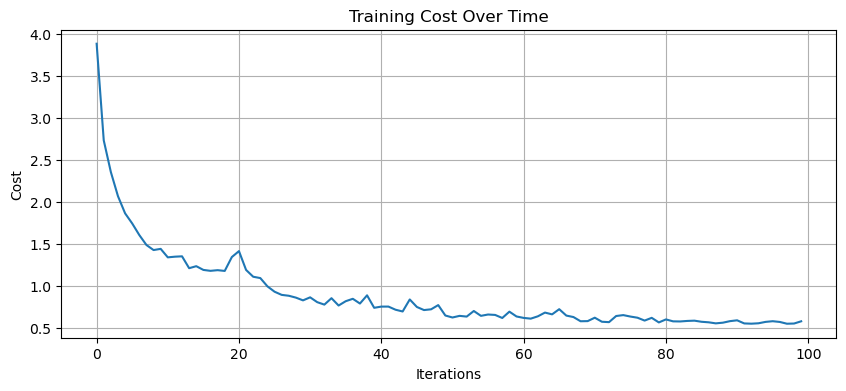
\includegraphics[width=0.8\textwidth]{cost_over_time.png}
\end{frame}

\begin{frame}{Performance Analysis}
    \begin{itemize}
        \item \textbf{Overall Metrics}
        \begin{itemize}
            \item Test Accuracy: 77.36\%
            \item Weighted F1-score: 0.77
            \item Macro F1-score: 0.75
        \end{itemize}
        \item \textbf{Best Performing Letters (F1-score)}
        \begin{itemize}
            \item O: 1.00
            \item B: 0.96
            \item C: 0.96
            \item A: 0.94
        \end{itemize}
        \item \textbf{Challenging Letters (F1-score)}
        \begin{itemize}
            \item R: 0.46
            \item Q: 0.55
            \item M: 0.57
            \item S: 0.57
        \end{itemize}
    \end{itemize}
\end{frame}

\begin{frame}{Confusion Matrix}
    \centering
    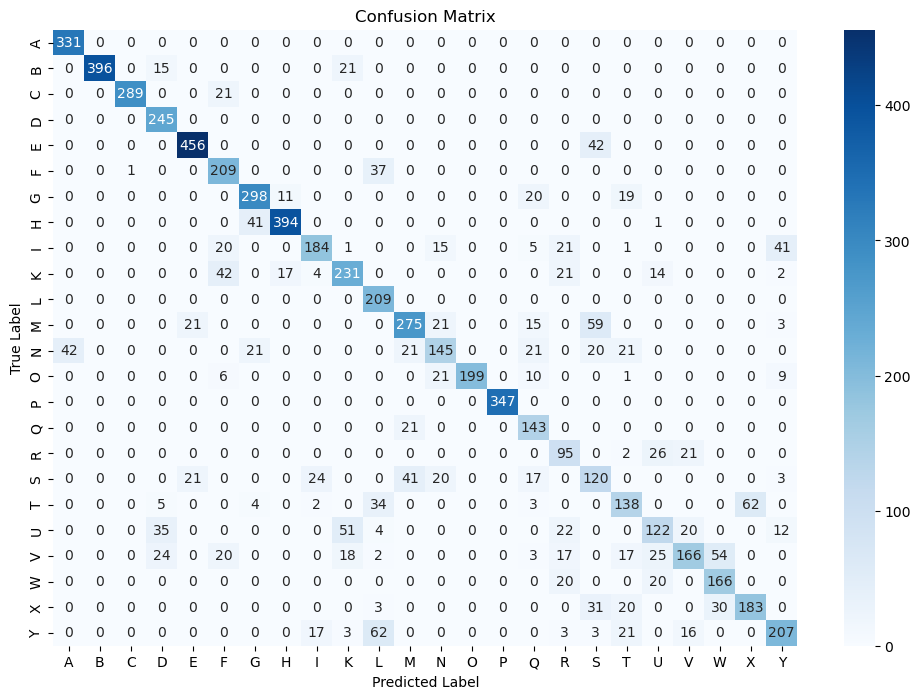
\includegraphics[width=0.8\textwidth]{confusion.png}
\end{frame}

\begin{frame}{Interactive Web Implementation}
    \begin{itemize}
        \item \textbf{User Interface:}
            \begin{minipage}{\textwidth}
                \begin{columns}[t]
                    \begin{column}{0.45\textwidth}
                        \begin{itemize}
                            \item Live webcam feed
                            \item Image capture functionality
                            \item Preview of original capture
                        \end{itemize}
                    \end{column}
                    \begin{column}{0.45\textwidth}
                        \begin{itemize}
                            \item Processed 28×28 preview
                            \item Top-3 predictions display
                            \item Confidence percentages
                        \end{itemize}
                    \end{column}
                \end{columns}
            \end{minipage}
        \vspace{0.25cm}

        \item \textbf{Processing Pipeline:}
            \begin{itemize}
                \item Real-time grayscale conversion
                \item Size normalization to 28×28
                \item Pixel value normalization (0-1 range)
            \end{itemize}
        \vspace{0.25cm}

        \item \textbf{Network Visualization:}
            \begin{itemize}
                \item Layer-by-layer activation monitoring
                \item Neuron activity visualization
                \item Confidence distribution display
            \end{itemize}
    \end{itemize}
\end{frame}

\section{Future Work}

\begin{frame}{Improvements \& Extensions}
    \begin{itemize}
        \item \textbf{Model Enhancements}
        \begin{itemize}
            \item Data augmentation for underrepresented classes
            \item Feature engineering for hand shape detection
            \item Deeper architecture exploration
        \end{itemize}
        \item \textbf{Practical Applications}
        \begin{itemize}
            \item Real-time recognition system
            \item Mobile application development
            \item Educational tools
        \end{itemize}
        \item \textbf{Research Extensions}
        \begin{itemize}
            \item Dynamic gesture recognition
            \item Multi-modal approaches
            \item Transfer learning exploration
        \end{itemize}
    \end{itemize}
\end{frame}

\begin{frame}{Conclusion}
    \begin{itemize}
        \item \textbf{Key Achievements}
        \begin{itemize}
            \item Successful static gesture recognition
            \item Balanced performance-complexity trade-off
            \item Identified clear paths for improvement
        \end{itemize}
        \item \textbf{Impact}
        \begin{itemize}
            \item Foundation for accessible communication tools
            \item Benchmark for future implementations
            \item Insights for sign language recognition systems
        \end{itemize}
    \end{itemize}
\end{frame}

\end{document}
